%! Licence = CC BY-NC-SA 4.0

%! Author = mariuszindel
%! Date = 06. Jul 2021
%! Project = DS1-Summary


\section{Network protocols}

\subsection{OSI-Layer}

\begin{center}
    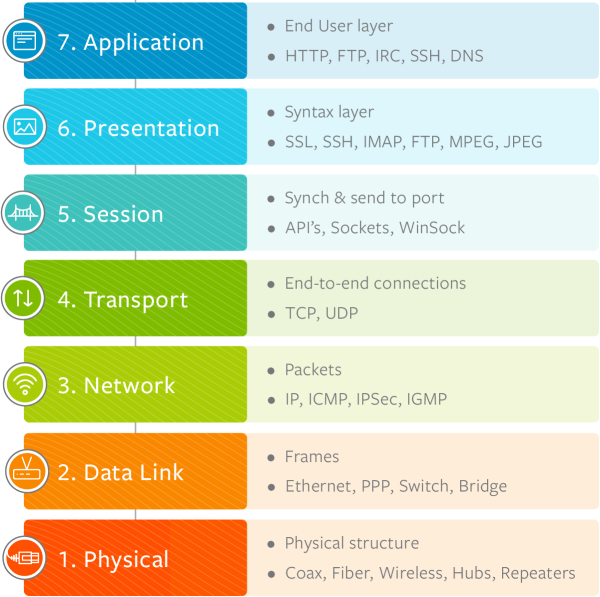
\includegraphics[scale=.25]{02-Protocols/osi-model.png}
    \vspace{-8pt}
\end{center}

\subsection{Layer Abstraction}
\begin{itemize}
    \item Protocols enable an entity to interact with an entity at the same layer in another host
    \item \textbf{Service definitions:} provide functionality to an (N)-layer by an (N-1) layer
    \item Layer N exchange protocol data units (PDUs) with layer N protocol
    \item Each PDU contains a header and payload, the service data unit (SDU)
\end{itemize}
\vspace{-8pt}
\begin{center}
    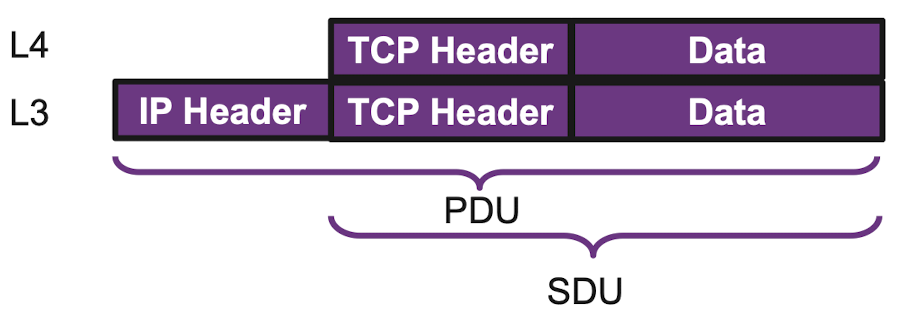
\includegraphics[scale=.3]{02-Protocols/Layer-abstraction.png}
\end{center}
\vspace{-8pt}

\subsection{Layer 4 - Transport Layer}

\subsubsection{TCP (Transmission Control Protocol)}
\begin{itemize}
    \item Reliable
    \item Ordered
    \item Window - capacity of receiver
    \item Checksum - 16bit
    \item TCP overhead: 20 bytes
    \item Tries to correct errors
\end{itemize}

\paragraph{Connection establishment}
\begin{itemize}
    \item SYN, SYN-ACK, ACK
    \item Initiates TCP session: initial sequence number is random
\end{itemize}
\paragraph{Connection termination}
\begin{itemize}
    \item FIN, ACK + FIN, ACK
    \item 3-way handshake
\end{itemize}
\paragraph{Sequences and ACKs}
\begin{itemize}
    \item Identification each byte of data
    \item Order of the bytes: reconstruction
    \item Detecting lost data: RTO, DupACK
\end{itemize}
\paragraph{Retransmission timeout}
\begin{itemize}
    \item If no ACK is received after timeout
\end{itemize}
\paragraph{Flow control}
\begin{itemize}
    \item Sender is not overwhelming a receiver
    \item Back pressure
    \item Sliding window
    \item Congestion control
    \begin{itemize}
        \item Slow-start
        \item Congestion avoidance
    \end{itemize}
\end{itemize}

\subsubsection{TCP + TLS}
\begin{center}
    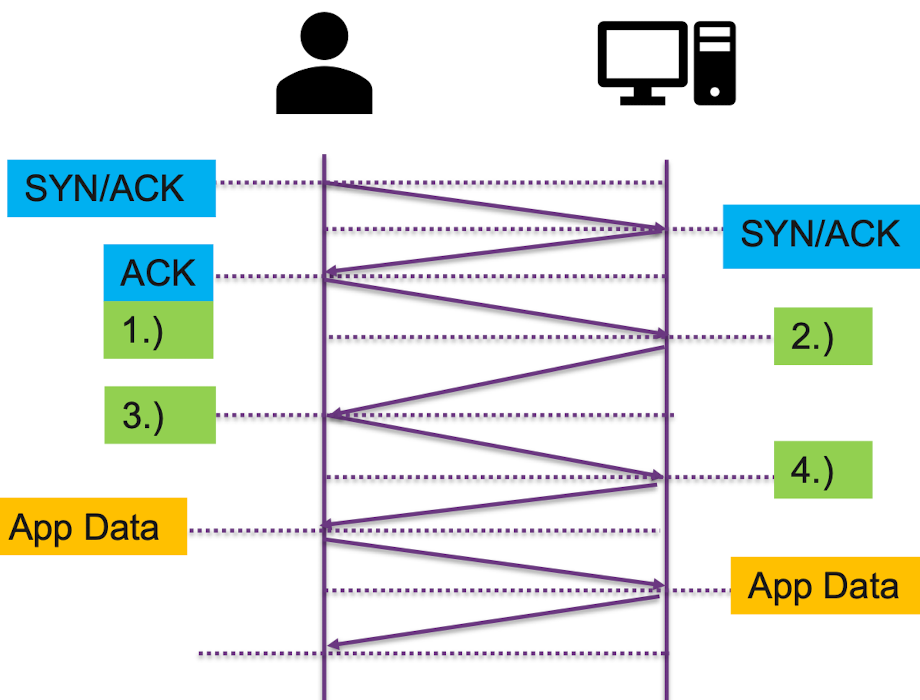
\includegraphics[scale=.3]{02-Protocols/TCP-TLS.png}
\end{center}
\begin{enumerate}
    \item \textbf{client hello:} lists crypto information, TLS version, ciphers/keys
    \item \textbf{server hello:} chosen cipher, session ID, random bytes, digital certificate
    \item \textbf{Key exchange:} using random bytes, now client + server can calculate secret key
    \item \textbf{finished:} encrypted message
\end{enumerate}
\paragraph{TLS 1.3}
1 RTT instead of 2
\begin{enumerate}
    \item Client Hello + Key share
    \item Server Hello + Key share + Verify Certificate + Finished
\end{enumerate}
0 RTT possible for previous connections (no perfect forward secrecy)

\subsubsection{QUIC (Quick UDP Internet Connections)}
\begin{itemize}
    \item 1 RTT (0 RTT for know connections)
    \item Built in security
\end{itemize}
\begin{center}
    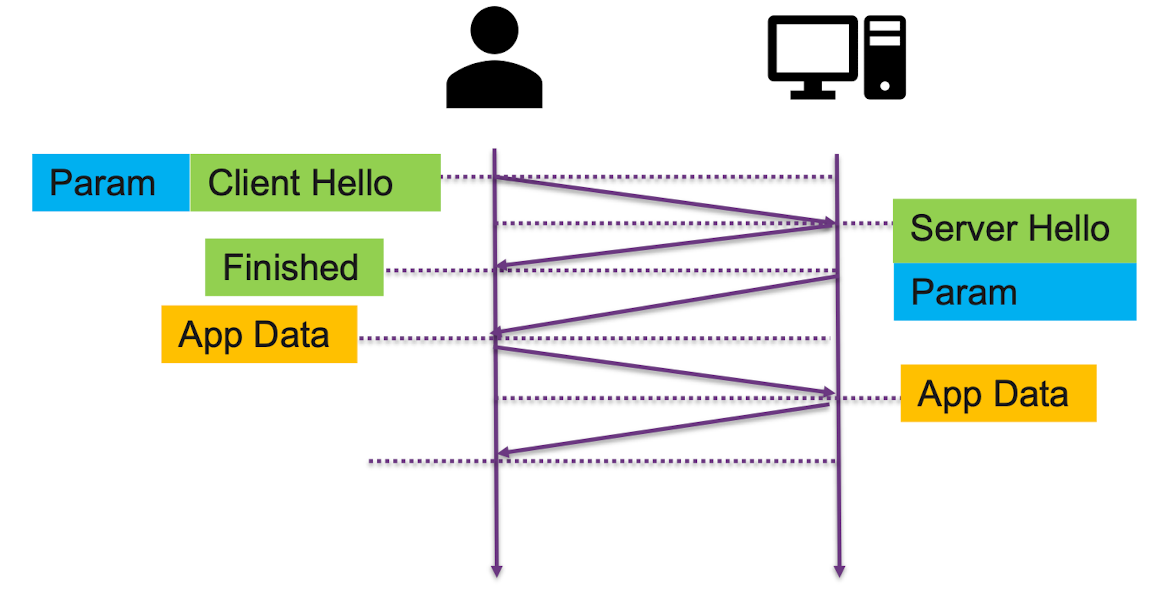
\includegraphics[scale=.25]{02-Protocols/quic.png}    
\end{center}
\begin{itemize}
    \item Multiplexing in HTTP/2
    \item QUIC can multiplex requests: one stream does not affect others
\end{itemize}

\subsubsection{UDP (User Datagram Protocol)}
\begin{itemize}
    \item Used for DNS, streaming
    \item Connection less
    \item No guarantee
    \begin{itemize}
        \item Delivery
        \item Ordering
        \item Duplicate protection
    \end{itemize}
    \item Lightweight
    \item Unordered
    \item No flow, congestion 
    \item Error checking, no recovery
\end{itemize}

\subsubsection{UDP (User Datagram Protocol)}
\begin{itemize}
    \item Connection oriented
    \item used in WebRTC 
    \item Reliable transfer 
    \item Messages 
    \item User can choose order
    \item Flow and congestion control 
    \item Heavyweight
    \item Error checking and recovery
\end{itemize}
\vfill
$ $
\columnbreak
